\documentclass[a4paper,11pt]{article}

% Packages
\usepackage[utf8]{inputenc}
\usepackage{amsmath}
\usepackage{graphicx}
\usepackage{geometry}
\usepackage{enumitem}
\geometry{a4paper, margin=1in}

% Title and Author
\title{Project 2}
\author{Ahmed Tlili, Leon Petrinos, Mathilde Peruzzo}
\date{\today}

\begin{document}

\maketitle

\section{ER Diagram}
\begin{figure}[h]
    \centering
    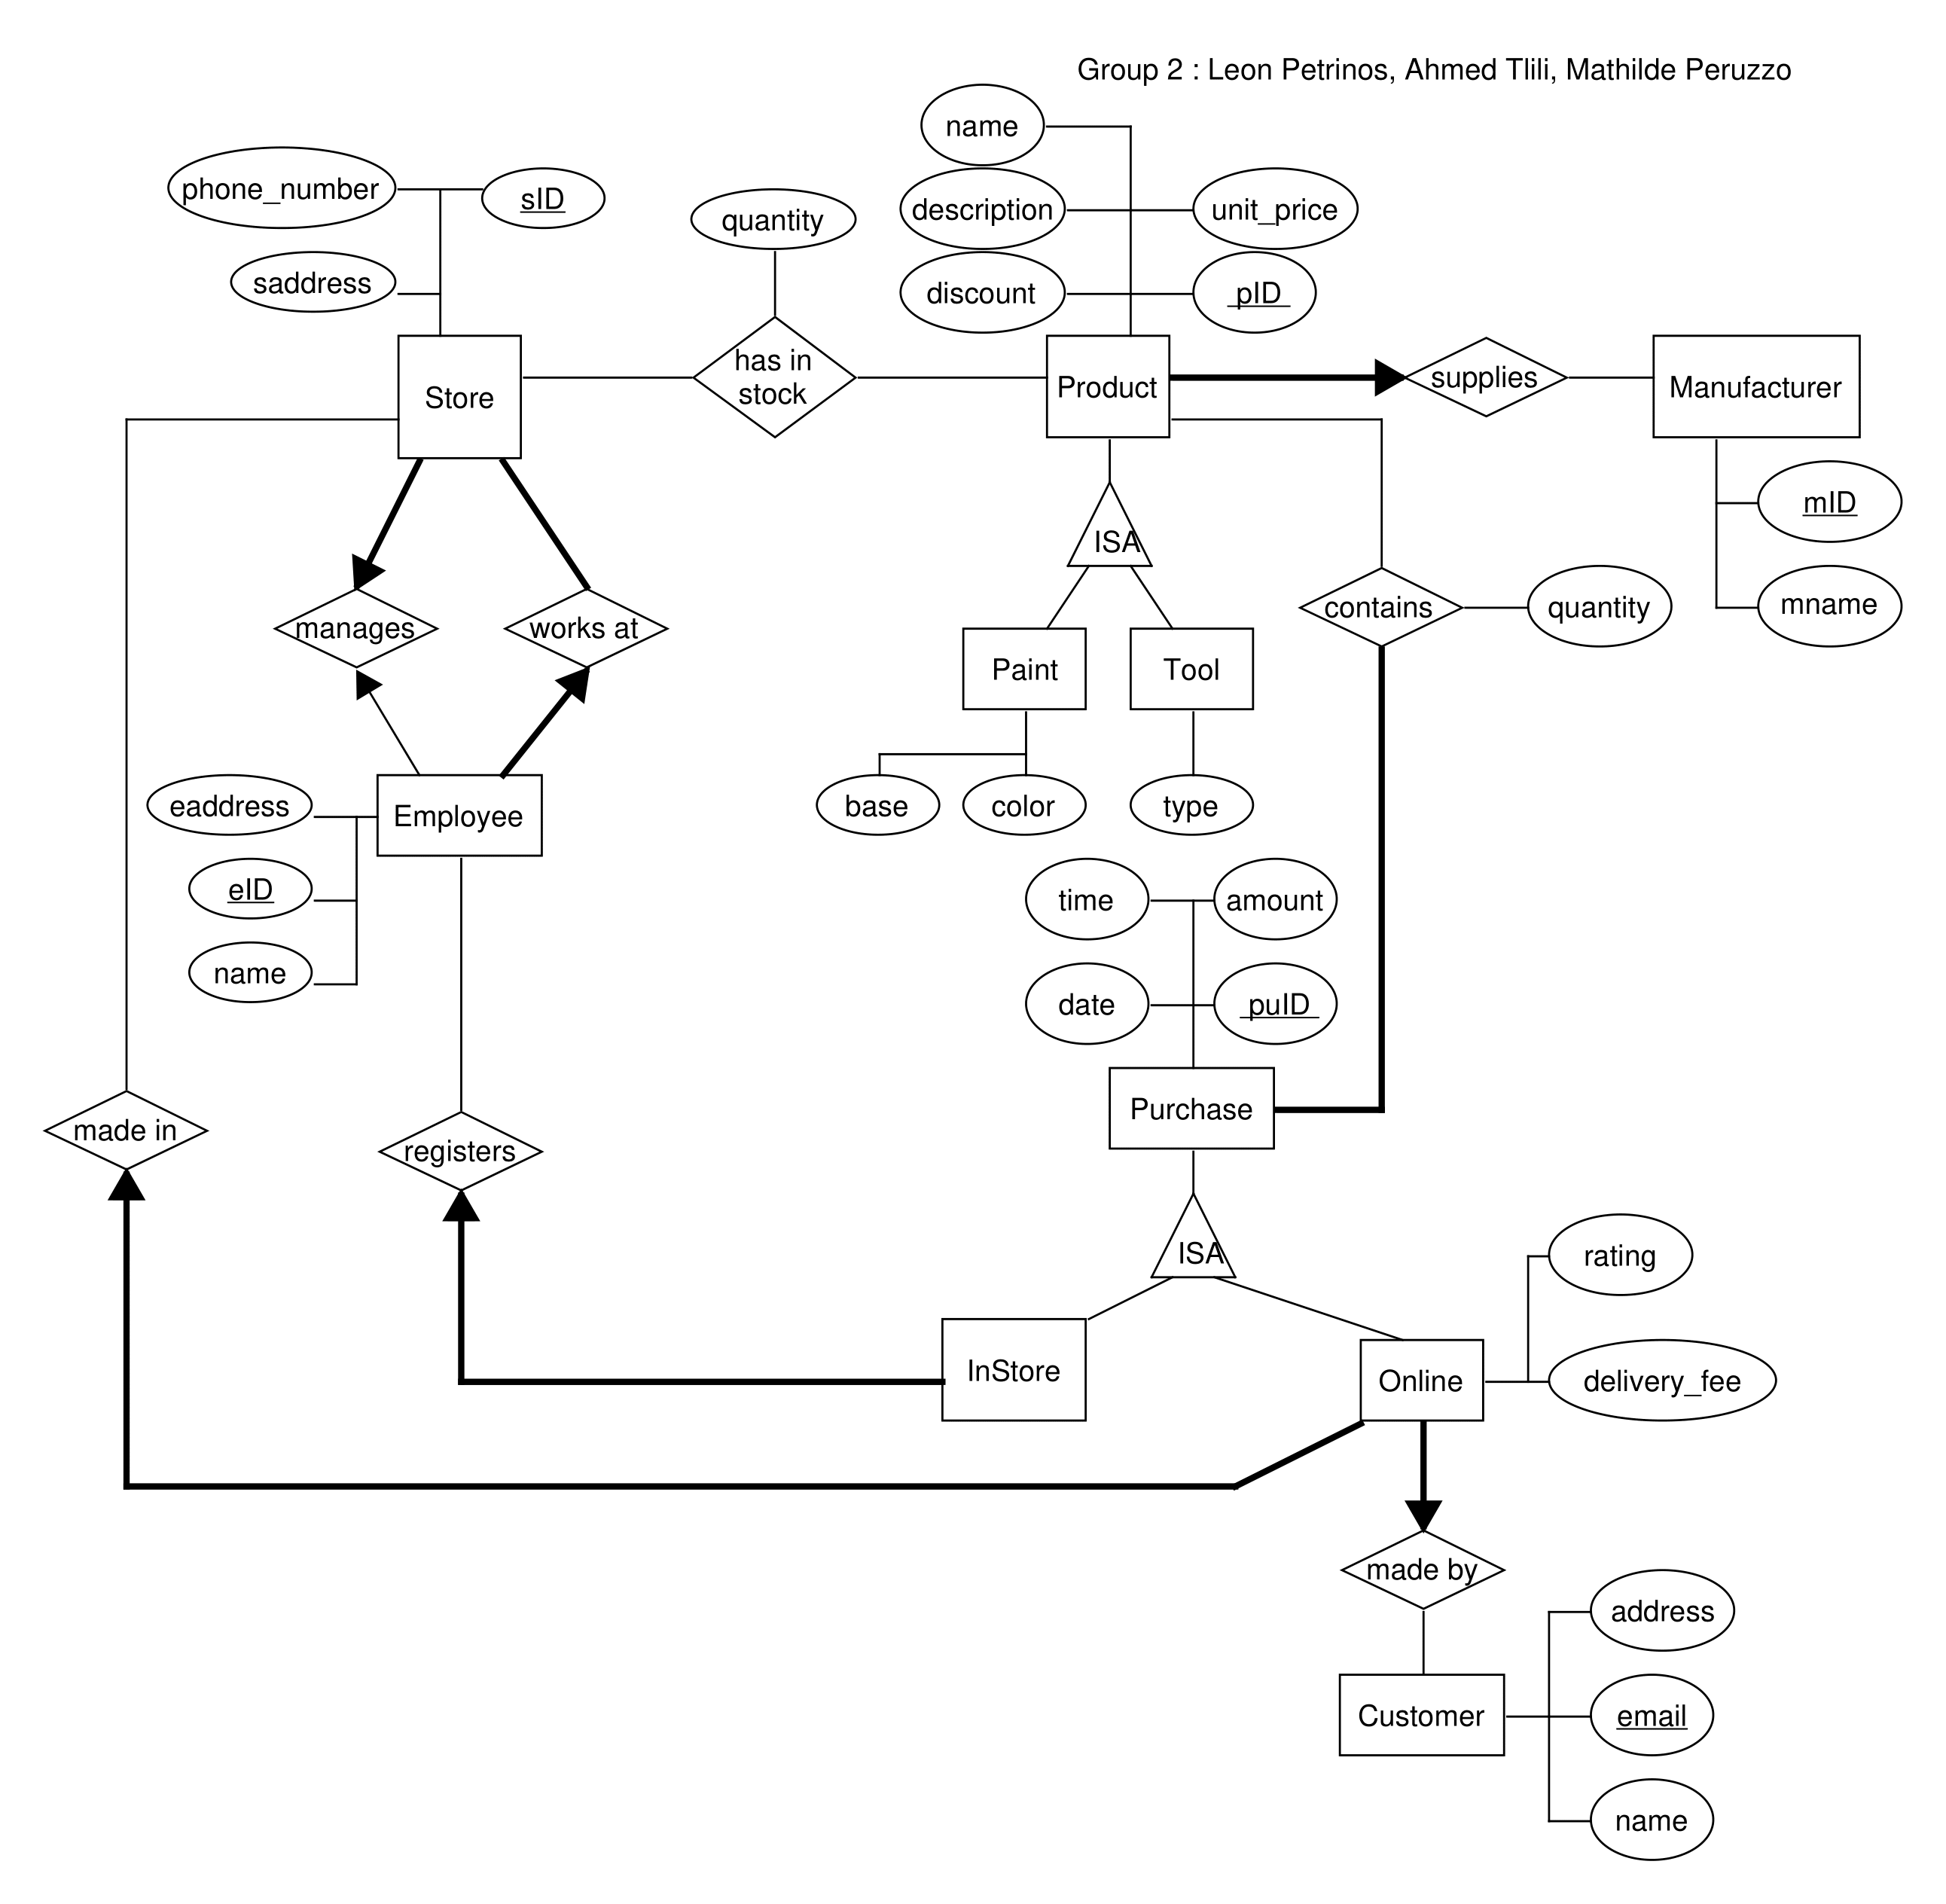
\includegraphics[width=0.8\textwidth]{ER.png}
    \caption{ER Diagram}
\end{figure}

\section{Relational Schema}
\begin{itemize}
    \item \textbf{Store}(\underline{s\_id}, s\_address, phone\_number, manager\_id UNIQUE NOT NULL)\\
        FOREIGN KEY(manager\_id) REFERENCES Employee(employee\_id)
    \item \textbf{Employee}(\underline{e\_id}, e\_name, s\_id)\\
        FOREIGN KEY(s\_id) REFERENCES Store(s\_id)
    \item \textbf{Manufacturer}(\underline{m\_id}, m\_name)
    \item \textbf{Product}(\underline{p\_id}, p\_name NOT NULL, unit\_price NOT NULL, description,\\ discount\_percentage, m\_id NOT NULL)\\
        FOREIGN KEY(m\_id) REFERENCES Manufacturer(m\_id)
    \item \textbf{Paint}(\underline{p\_id}, base, color)\\
        FOREIGN KEY(p\_id) REFERENCES Product(p\_id)
    \item \textbf{Tool}(\underline{p\_id}, type)
    \item \textbf{Has\_in\_stock}(\underline{p\_id}, \underline{s\_id}, quantity NOT NULL CHECK(quantity $\geq$ 0))\\
        FOREIGN KEY(p\_id) REFERENCES Product(p\_id)\\
        FOREIGN KEY(s\_id) REFERENCES Store(s\_id)
    \item \textbf{Customer}(\underline{email}, c\_name, c\_address NOT NULL)\\
        PRIMARY KEY(email)
    \item \textbf{Purchase}(\underline{p\_id}, amount NOT NULL, p\_date NOT NULL, p\_time NOT NULL)
    \item \textbf{Contains\_purchase}(\underline{p\_id}, \underline{product\_id}, quantity NOT NULL CHECK(quantity $\geq$ 0))\\
        FOREIGN KEY(p\_id) REFERENCES Purchase(p\_id)\\
        FOREIGN KEY(product\_id) REFERENCES Product(p\_id)
    \item \textbf{Instore}(\underline{p\_id}, \underline{e\_id})\\
        FOREIGN KEY(p\_id) REFERENCES Purchase(p\_id)\\
        FOREIGN KEY(e\_id) REFERENCES Employee(e\_id)
    \item \textbf{Online}(\underline{p\_id}, rating CHECK(rating $\geq$ 0 AND rating $\leq$ 5 OR rating IS NULL), delivery\_fee NOT NULL, email NOT NULL)\\
        FOREIGN KEY(p\_id) REFERENCES Purchase(p\_id)\\
        FOREIGN KEY(email) REFERENCES Customer(email)


\end{itemize}

\section{Pending Constraints}
\begin{itemize}
    \item A store should have at least one employee. (TODO: might not be correct as a every store should have a manage which will work there as well)
    \item A purchase should have at least one product.
    \item Cannot have store manager\_id referencing a row in the Employee table.\\
        As here we have two tables referencing each other (STORE, EMPLOYEE).\\
        One of them has to drop the foreign key constraint.
        % -- Add STORE constraint after EMPLOYEE table is created
        % ALTER TABLE STORE
        % ADD CONSTRAINT FK_store_manager FOREIGN KEY(manager_id) REFERENCES EMPLOYEE(e_id);

\end{itemize}


\end{document}

